\chapter{Bilans thermodynamiques et systèmes ouverts}\label{ch:b2:open-systems}

La thermodynamique du volume de première année traitait de systèmes fermés ---
une masse fixe de gaz dans un cylindre, comprimée, chauffée, détendue. Mais
les machines qui chauffent réellement nos maisons, refroidissent nos aliments et font notre
électricité sont traversées par un \emph{écoulement}~: la vapeur file à travers la
turbine d'une centrale à des centaines de kilogrammes par seconde, un
fluide frigorigène circule dans le compresseur, le condenseur, le \omterm{prop:b2:open-systems:devices}{détendeur} et
l'évaporateur d'une pompe à chaleur, l'air traverse le compresseur et la
chambre de combustion d'un réacteur. Chaque organe est un \emph{\omterm{def:b2:open-systems:cv}{système
ouvert}}, une région de l'espace où de la matière entre et sort, et les
premier et second principes doivent être réécrits pour lui. La réécriture est brève
--- la clé est que le fluide poussé dans le système emporte, outre
son énergie interne, le travail fourni pour l'y pousser, et c'est pourquoi
l'\emph{\omterm{thm:b2:open-systems:firstlaw}{enthalpie}}, et non l'énergie interne, est l'énergie naturelle d'un écoulement.
Ce chapitre établit les bilans de masse, d'énergie et d'entropie pour les
\omterm{def:b2:open-systems:cv}{systèmes ouverts} en régime \omterm{def:b2:open-systems:cv}{permanent}, les applique aux organes élémentaires ---
\omterm{prop:b2:open-systems:devices}{tuyère}, \omterm{prop:b2:open-systems:devices}{détendeur}, compresseur, turbine, échangeur --- et assemble
ces organes en les deux cycles que dimensionne le problème du week-end~: une
pompe à chaleur et une centrale à vapeur.

\begin{omfigure}
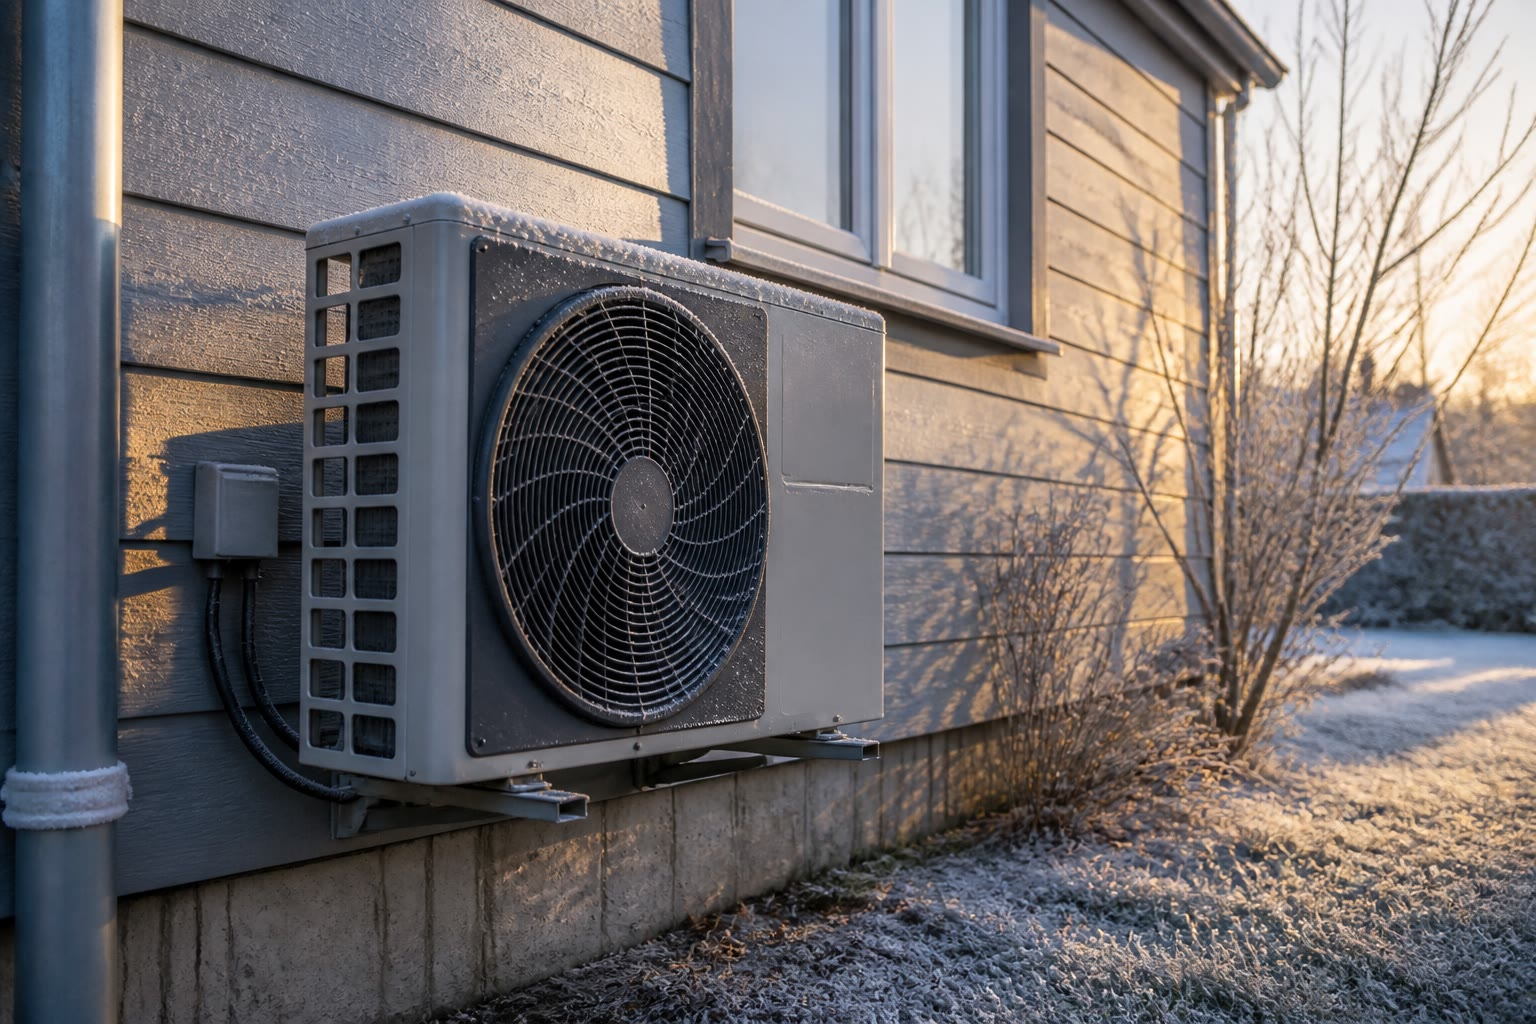
\includegraphics[width=0.58\linewidth]{images/book4/ai/b4-27-heat-pump-winter.jpg}

{\small L'unité extérieure d'une pompe à chaleur par un matin d'hiver~: un ventilateur
tire l'air froid sur l'évaporateur, et à l'intérieur un compresseur, un
condenseur et un \omterm{prop:b2:open-systems:devices}{détendeur} transportent cette chaleur, multipliée par trois ou quatre,
jusque dans la maison.}
\end{omfigure}

\section{Systèmes ouverts et bilan de masse}

\begin{definition}[Système ouvert, volume de contrôle, régime permanent]\label{def:b2:open-systems:cv}
Un \emph{système ouvert}\index{système ouvert} est une région fixe de l'espace,
le \emph{volume de contrôle}\index{volume de contrôle} $\Sigma$, limité par une
surface à travers laquelle du fluide entre et sort (sections d'entrée et de
sortie) et à travers laquelle chaleur et travail peuvent être échangés avec
l'extérieur~; le travail reçu par des pièces mobiles (un arbre, un piston)
autres que l'écoulement lui-même est le \emph{travail utile}\index{travail utile}
$W_{\text{u}}$ (travail d'arbre). L'écoulement est \emph{permanent}\index{régime permanent (écoulement)} quand tout champ à l'intérieur de $\Sigma$ est indépendant du temps~: la masse,
l'énergie et l'entropie contenues dans $\Sigma$ sont alors constantes.
\end{definition}

\begin{proposition}[Bilan de masse]\label{prop:b2:open-systems:mass}
À travers une section d'aire $S$ où le fluide de masse volumique $\rho$ se déplace
à la vitesse moyenne $c$ normale à elle passe le \emph{débit
massique}\index{débit massique} $\dot m = \rho c S$ (en \unit{kg/s}). En
régime \omterm{def:b2:open-systems:cv}{permanent}, ce qui entre sort~: $\sum_{\text{e}}\dot m = \sum_{\text{s}}
\dot m$~; pour un écoulement unique, $\dot m$ est le même à l'entrée et à la sortie,
$\rho_1c_1S_1 = \rho_2c_2S_2$ --- l'\omterm{thm:b2:fluid-kinematics:continuity}{équation de continuité} du
\cref{ch:b2:fluid-kinematics} intégrée sur la section.
\end{proposition}

\begin{proof}
La masse dans $\Sigma$ est constante, donc les flux s'équilibrent.
\end{proof}

\section{Le premier principe pour un système ouvert}

\begin{theorem}[Bilan d'énergie d'un écoulement permanent à une entrée et une sortie]\label{thm:b2:open-systems:firstlaw}
Pour un écoulement \omterm{def:b2:open-systems:cv}{permanent} de \omterm{def:b2:fluid-kinematics:flowrate}{débit massique} $\dot m$ entrant dans l'état 1
et sortant dans l'état 2, recevant la puissance utile (d'arbre)
$P_{\text{u}}$ et la puissance thermique $P_{\text{th}}$,
\[
\dot m\,\Big[(h_2 - h_1) + \tfrac12(c_2^2 - c_1^2) + g(z_2 - z_1)\Big]
= P_{\text{u}} + P_{\text{th}} ,
\]
ou, par unité de masse de fluide traversant le système,
\[
\Delta h + \Delta\big(\tfrac12c^2\big) + g\,\Delta z = w_{\text{u}} + q .
\]
L'\emph{enthalpie}\index{enthalpie (écoulement)} $h = u + Pv$ remplace
l'énergie interne~: $Pv$ est le \emph{travail de transvasement}, le travail fourni par
le fluide amont pour pousser une unité de masse à l'intérieur, moins celui fourni pour la pousser
au-dehors.
\end{theorem}

\begin{proof}
Suivons le système fermé formé du fluide contenu dans $\Sigma$ à l'instant $t$ plus
la tranche $\dd m = \dot m\,\dd t$ sur le point d'entrer~; à $t + \dd t$ il se
compose du fluide contenu dans $\Sigma$ (même état, régime \omterm{def:b2:open-systems:cv}{permanent}) plus la
tranche $\dd m$ qui est sortie. Son énergie a varié de
$\dd m\,[(u_2 + \tfrac12c_2^2 + gz_2) - (u_1 + \tfrac12c_1^2 + gz_1)]$. Il a
reçu $P_{\text{u}}\dd t + P_{\text{th}}\dd t$, plus le travail des
forces de pression à l'entrée, $P_1S_1 \times c_1\dd t = P_1v_1\,\dd m$
(pour pousser la tranche à l'intérieur), moins celui à la sortie, $P_2v_2\,\dd m$. Le
premier principe pour ce système fermé, avec $u + Pv = h$, donne le résultat.
\end{proof}

\begin{omfigure}
\begin{tikzpicture}[scale=0.95, >=stealth]
  \draw[thick, rounded corners=6pt, fill=omDef!8] (1.2,0) rectangle (6.2,2.6);
  \node[font=\scriptsize] at (3.7,1.9) {volume de contrôle $\Sigma$ (permanent)};
  % inlet pipe
  \draw[thick] (-0.6,0.5) -- (1.2,0.5); \draw[thick] (-0.6,1.1) -- (1.2,1.1);
  \fill[omExo!40] (-0.5,0.52) rectangle (0.1,1.08);
  \node[font=\scriptsize, above] at (-0.2,1.12) {$\dd m$};
  \draw[->, omExo, thick] (-1.4,0.8) -- (-0.6,0.8);
  \node[font=\scriptsize, left] at (-1.4,0.8) {$\dot m$, $h_1$, $c_1$, $z_1$};
  % outlet pipe
  \draw[thick] (6.2,1.5) -- (8.0,1.5); \draw[thick] (6.2,2.1) -- (8.0,2.1);
  \fill[omExo!40] (7.3,1.52) rectangle (7.9,2.08);
  \node[font=\scriptsize, above] at (7.6,2.12) {$\dd m$};
  \draw[->, omExo, thick] (8.0,1.8) -- (8.8,1.8);
  \node[font=\scriptsize, right] at (8.8,1.8) {$h_2$, $c_2$, $z_2$};
  % shaft
  \draw[->, omThm, very thick] (3.7,-0.8) -- (3.7,0) node[pos=0, below, font=\scriptsize] {$P_{\text{u}}$ (arbre)};
  \draw[->, omThm, very thick] (5.5,3.4) -- (5.5,2.6) node[pos=0, above, font=\scriptsize] {$P_{\text{th}}$};
  % pressure pushes
  \node[font=\scriptsize, omExo] at (0.3,0.2) {$P_1v_1$ pousse dedans};
  \node[font=\scriptsize, omExo] at (7.2,1.2) {$P_2v_2$ pousse dehors};
\end{tikzpicture}

{\small Le \omterm{def:b2:open-systems:cv}{système ouvert} \omterm{def:b2:open-systems:cv}{permanent}~: le système fermé que l'on suit pendant $\dd
t$ est le contenu de $\Sigma$ plus la tranche entrante, puis le contenu
plus la tranche sortante~; le travail des pressions aux deux sections change $u$
en $h = u + Pv$.}
\end{omfigure}

\begin{remark}[Se servir du premier principe]\label{rem:b2:open-systems:using}
Pour un gaz parfait $\Delta h = c_p\Delta T$~; pour un liquide $\Delta h \approx
c\,\Delta T + v\,\Delta P$ (le second terme est le travail de la pompe)~; pour une vapeur
on lit $h$ dans des tables ou sur des diagrammes. Le terme cinétique est en général
négligeable~: à \qty{10}{m/s}, $c^2/2 = \qty{50}{J/kg}$, contre
\qty{1}{kJ/kg} pour un kelvin d'air --- il ne compte que dans les \omterm{prop:b2:open-systems:devices}{tuyères} et les
aubes de turbine, où les vitesses atteignent des centaines de mètres par seconde. Le
terme de pesanteur, $g\Delta z \approx \qty{10}{J/kg}$ par mètre, compte pour
l'eau d'un barrage, jamais dans un cycle à gaz. Avec plusieurs entrées et sorties
le bilan s'écrit $\sum_{\text{s}}\dot m\,h - \sum_{\text{e}}\dot m\,h =
P_{\text{u}} + P_{\text{th}}$ (termes cinétique et de pesanteur négligés).
\end{remark}

\section{Le second principe pour un système ouvert}

\begin{theorem}[Bilan d'entropie d'un écoulement permanent]\label{thm:b2:open-systems:secondlaw}
Pour un écoulement \omterm{def:b2:open-systems:cv}{permanent} à une entrée et une sortie échangeant les puissances thermiques
$P_{\text{th},i}$ avec des sources aux températures $T_i$,
\[
\dot m\,(s_2 - s_1) = \sum_i\frac{P_{\text{th},i}}{T_i} + \dot S_{\text{c}},
\qquad \dot S_{\text{c}} \ge 0 ;
\]
par unité de masse, $\Delta s = s_{\text{éch}} + s_{\text{c}}$. Un écoulement adiabatique
réversible est \emph{isentropique}~; un écoulement adiabatique réel a $s_2 >
s_1$. Le \emph{rendement isentropique}\index{rendement isentropique}
d'une turbine vaut $\eta_{\text{T}} = w_{\text{réel}}/w_{\text{s}} = (h_1 - h_2)/(h_1
- h_{2s})$ et celui d'un compresseur $\eta_{\text{C}} = (h_{2s} - h_1)/(h_2 -
h_1)$, où $2s$ est l'état atteint isentropiquement à la même
pression de sortie~; tous deux valent typiquement $0.8$--$0.9$. Le travail perdu par
irréversibilité, rapporté à la température ambiante $T_0$, vaut
$T_0\,s_{\text{c}}$ par unité de masse.
\end{theorem}

\begin{proof}
Même système fermé que plus haut~: son entropie varie de $\dd m\,(s_2 -
s_1)$, il reçoit $\sum P_{\text{th},i}\dd t/T_i$ des sources, et le
reste est créé.
\end{proof}

\section{Les organes élémentaires}

\begin{proposition}[Tuyère, détendeur, compresseur, turbine, échangeur]\label{prop:b2:open-systems:devices}
Tous adiabatiques sauf mention contraire, en régime \omterm{def:b2:open-systems:cv}{permanent}, termes cinétique et de pesanteur
négligés sauf s'ils sont l'objet même.
\begin{itemize}
\item \emph{Tuyère}\index{tuyère} (pas d'arbre, pas de chaleur)~: $\tfrac12c_2^2 -
      \tfrac12c_1^2 = h_1 - h_2$ --- l'\omterm{thm:b2:open-systems:firstlaw}{enthalpie} devient vitesse~; un
      \emph{diffuseur} fait l'inverse.
\item \emph{Détendeur}\index{détendeur} (vanne, bouchon poreux~; pas d'arbre,
      pas de chaleur, vitesses faibles)~: $h_2 = h_1$, \emph{isenthalpique}. Pour un
      gaz parfait $T_2 = T_1$~; pour un gaz réel la température baisse en général
      (effet Joule--Thomson)~; pour un liquide près de la saturation une
      fraction se vaporise brusquement --- le \omterm{prop:b2:open-systems:devices}{détendeur} de tout réfrigérateur.
\item \emph{Compresseur, pompe, turbine}\index{turbine} (machines
      adiabatiques)~: $w_{\text{u}} = h_2 - h_1$ --- positif pour un compresseur,
      négatif pour une turbine~; pour une pompe à liquide $w_{\text{u}} \approx
      v(P_2 - P_1)$, minuscule parce que $v$ est petit.
\item \emph{Échangeur de chaleur}\index{échangeur de chaleur} (deux courants, pas
      d'arbre, adiabatique dans son ensemble)~: $\dot m_{\text{a}}(h_{\text{a},2} -
      h_{\text{a},1}) = -\dot m_{\text{b}}(h_{\text{b},2} - h_{\text{b},1})$
      --- ce que l'un perd l'autre le gagne~; l'échange crée de l'entropie
      à moins que les courants ne soient partout à la même température
      (le contre-courant la réduit).
\item \emph{Chambre de mélange}~: $\sum\dot m_{\text{e}}h_{\text{e}} = \dot
      m_{\text{s}}h_{\text{s}}$.
\end{itemize}
\end{proposition}

\begin{proof}
Chacun est le premier principe avec les termes voulus mis à zéro.
\end{proof}

\begin{omfigure}
\begin{tikzpicture}[scale=0.85, >=stealth]
  % nozzle
  \draw[thick] (0,0.2) -- (1.6,0.55) -- (1.6,0.85) -- (0,1.2);
  \draw[->, omExo, thick] (-0.6,0.7) -- (-0.1,0.7);
  \draw[->, omExo, very thick] (1.7,0.7) -- (2.9,0.7);
  \node[font=\scriptsize] at (1.0,-0.35) {tuyère~: $h \to c^2/2$};
  % throttle
  \begin{scope}[xshift=4.6cm]
    \draw[thick] (0,0.4) -- (1.0,0.4) -- (1.0,0.55) -- (1.2,0.55) -- (1.2,0.4) -- (2.4,0.4);
    \draw[thick] (0,1.0) -- (1.0,1.0) -- (1.0,0.85) -- (1.2,0.85) -- (1.2,1.0) -- (2.4,1.0);
    \draw[->, omExo, thick] (-0.6,0.7) -- (-0.1,0.7);
    \draw[->, omExo, thick] (2.5,0.7) -- (3.1,0.7);
    \node[font=\scriptsize] at (1.2,-0.35) {détendeur~: $h_2 = h_1$};
    \node[font=\scriptsize] at (0.4,1.3) {$P_1$}; \node[font=\scriptsize] at (2.0,1.3) {$P_2 < P_1$};
  \end{scope}
  % turbine
  \begin{scope}[xshift=9.6cm]
    \draw[thick] (0,1.3) -- (0,0.1) -- (2.0,-0.3) -- (2.0,1.7) -- cycle;
    \draw[->, omExo, thick] (-0.7,1.0) -- (-0.1,1.0);
    \draw[->, omExo, thick] (2.1,0.3) -- (2.8,0.3);
    \draw[->, omThm, very thick] (1.0,-0.4) -- (1.0,-1.0) node[below, font=\scriptsize] {$w_{\text{u}} = h_2 - h_1 < 0$};
    \node[font=\scriptsize] at (1.0,2.0) {turbine};
  \end{scope}
  % exchanger
  \begin{scope}[yshift=-3.2cm]
    \draw[thick, rounded corners=4pt] (0,0) rectangle (4.4,1.4);
    \draw[->, omExo, very thick] (-0.6,1.1) -- (0,1.1); \draw[omExo, very thick] (0,1.1) -- (4.4,1.1); \draw[->, omExo, very thick] (4.4,1.1) -- (5.0,1.1);
    \draw[<-, omDef, very thick] (-0.6,0.3) -- (0,0.3); \draw[omDef, very thick] (0,0.3) -- (4.4,0.3); \draw[<-, omDef, very thick] (4.4,0.3) -- (5.0,0.3);
    \node[font=\scriptsize, omExo, left] at (-0.6,1.1) {chaud entrant}; \node[font=\scriptsize, omExo, right] at (5.0,1.1) {chaud sortant};
    \node[font=\scriptsize, omDef, right] at (5.0,0.3) {froid entrant}; \node[font=\scriptsize, omDef, left] at (-0.6,0.3) {froid sortant};
    \node[font=\scriptsize] at (2.2,-0.4) {échangeur à contre-courant~: $\dot m_{\text{a}}\Delta h_{\text{a}} = -\dot m_{\text{b}}\Delta h_{\text{b}}$};
    \node[font=\scriptsize] at (8.4,0.7) {(la chambre de mélange~: $\sum\dot m_{\text{e}}h_{\text{e}} = \dot m_{\text{s}}h_{\text{s}}$)};
  \end{scope}
\end{tikzpicture}

{\small Les \omterm{def:b2:open-systems:cv}{systèmes ouverts} élémentaires~: chacun est le bilan d'énergie avec
les termes sans objet rayés --- pas d'arbre dans une \omterm{prop:b2:open-systems:devices}{tuyère} ni un \omterm{prop:b2:open-systems:devices}{détendeur},
pas de chaleur dans une turbine adiabatique, pas de chaleur nette pour un échangeur pris dans
son ensemble.}
\end{omfigure}

\begin{example}[Des nombres pour les organes]\label{ex:b2:open-systems:numbers}
De la vapeur entrant dans une \omterm{prop:b2:open-systems:devices}{tuyère} de turbine à $h = \qty{3000}{kJ/kg}$ et sortant
à \qty{2800}{kJ/kg} atteint $c = \sqrt{2 \times 200 \times 10^3} =
\qty{630}{m/s}$. De l'air comprimé adiabatiquement de \qty{1}{bar},
\qty{293}{K} à \qty{8}{bar}~: isentropiquement $T_2 = 293 \times 8^{0.286} =
\qty{531}{K}$ et $w = c_p\Delta T = \qty{239}{kJ/kg}$~; avec $\eta_{\text{C}} =
0.8$, \qty{299}{kJ/kg} et \qty{590}{K} --- d'où le refroidissement des compresseurs
entre étages. Un radiateur d'automobile évacuant \qty{42}{kW} d'une eau
refroidie de \qty{10}{K} (\qty{1}{kg/s}) réchauffe \qty{2.1}{kg/s} d'air de
\qty{20}{K}. Du frigorigène liquide à \qty{40}{\celsius} détendu à
\qty{0}{\celsius} arrive en brouillard avec $28\%$ de vapeur~: cette vaporisation
brusque est ce qui refroidit le liquide à la température de l'évaporateur.
\end{example}

\section{Cycles}

\begin{proposition}[Machine frigorifique à compression de vapeur et pompe à chaleur]\label{prop:b2:open-systems:fridge}
Un frigorigène circule à travers~: (1$\to$2) un compresseur adiabatique
qui porte la vapeur de la pression d'évaporation à la pression de
condensation, $w = h_2 - h_1$~; (2$\to$3) un condenseur où il cède
$q_{\text{cond}} = h_2 - h_3$ au côté chaud (la pièce pour une pompe à chaleur, la
cuisine pour un réfrigérateur) et qu'il quitte à l'état liquide~; (3$\to$4) un \omterm{prop:b2:open-systems:devices}{détendeur}, $h_4
= h_3$~; (4$\to$1) un évaporateur où il absorbe $q_{\text{evap}} = h_1 - h_4$
au côté froid. Les coefficients de performance valent
\[
\mathrm{COP}_{\text{froid}} = \frac{h_1 - h_4}{h_2 - h_1}, \qquad
\mathrm{COP}_{\text{chaud}} = \frac{h_2 - h_3}{h_2 - h_1} = \mathrm{COP}_{\text{froid}} + 1 ,
\]
majorés par ceux de Carnot $T_{\text{c}}/(T_{\text{h}} - T_{\text{c}})$ et
$T_{\text{h}}/(T_{\text{h}} - T_{\text{c}})$~; le cycle se lit le plus aisément sur
le diagramme $(\log P, h)$, où les deux échanges et le travail sont des
segments horizontaux.
\end{proposition}

\begin{proof}
Les quatre bilans du premier principe~; le bilan d'énergie du cycle entier
donne $q_{\text{cond}} = q_{\text{evap}} + w$, d'où la relation entre
les deux COP.
\end{proof}

\begin{omfigure}
\begin{tikzpicture}
  \begin{axis}[width=8.6cm, height=5.2cm, xmin=150, xmax=480, ymin=-0.1, ymax=1.5,
    axis x line=bottom, axis y line=left, xlabel={$h$ (\unit{kJ/kg})}, ylabel={$\log P$},
    xlabel style={at={(axis description cs:0.5,-0.12)}, anchor=north}, ytick=\empty, xtick={200,300,400}, clip=false]
    % saturation dome (schematic)
    \addplot[gray, thick, smooth] coordinates {(200,0.3) (215,0.55) (232,0.85) (256,1.1) (290,1.3) (330,1.38) (370,1.3) (405,1.1) (418,0.85) (418,0.55) (399,0.3)};
    % cycle
    \draw[omDef, very thick] (axis cs:256,1.1) -- (axis cs:256,0.3);
    \draw[omDef, very thick] (axis cs:256,0.3) -- (axis cs:399,0.3);
    \draw[omDef, very thick] (axis cs:399,0.3) -- (axis cs:433,1.1);
    \draw[omDef, very thick] (axis cs:433,1.1) -- (axis cs:256,1.1);
    \fill (axis cs:399,0.3) circle (1.5pt) node[below, font=\scriptsize] {1};
    \fill (axis cs:433,1.1) circle (1.5pt) node[above, font=\scriptsize] {2};
    \fill (axis cs:256,1.1) circle (1.5pt) node[above, font=\scriptsize] {3};
    \fill (axis cs:256,0.3) circle (1.5pt) node[below, font=\scriptsize] {4};
    \node[font=\scriptsize, omDef] at (axis cs:330,0.2) {évaporateur $q_{\text{evap}}$};
    \node[font=\scriptsize, omDef] at (axis cs:345,1.2) {condenseur $q_{\text{cond}}$};
    \node[font=\scriptsize, omDef, anchor=west] at (axis cs:418,0.68) {$w$};
    \node[font=\scriptsize, gray] at (axis cs:205,0.95) {liquide};
    \node[font=\scriptsize, gray] at (axis cs:450,0.5) {vapeur};
    \node[font=\scriptsize, gray] at (axis cs:330,0.75) {liquide + vapeur};
  \end{axis}
\end{tikzpicture}

{\small Le cycle à compression de vapeur sur le diagramme $(\log P, h)$~: le
condenseur et l'évaporateur sont des isobares dans la cloche, le \omterm{prop:b2:open-systems:devices}{détendeur} une
isenthalpe verticale, le compresseur une ligne oblique~; les longueurs des
segments horizontaux sont les chaleurs et le travail par kilogramme.}
\end{omfigure}

\begin{proposition}[Le cycle à vapeur (Rankine)]\label{prop:b2:open-systems:rankine}
L'eau circule à travers~: (1$\to$2) une pompe, $w_{\text{p}} \approx v(P_2 -
P_1)$, quelques \unit{kJ/kg}~; (2$\to$3) une chaudière à haute pression où elle
est chauffée, vaporisée et surchauffée, $q_{\text{e}} = h_3 - h_2$~;
(3$\to$4) une turbine qui détend la vapeur jusqu'à la pression du condenseur,
$w_{\text{t}} = h_3 - h_4$ (un millier de \unit{kJ/kg})~; (4$\to$1) un condenseur
à basse pression où la vapeur humide redevient liquide, rejetant
$q_{\text{s}} = h_4 - h_1$ à l'eau de refroidissement. Le rendement vaut
\[
\eta = \frac{w_{\text{t}} - w_{\text{p}}}{q_{\text{e}}} = 1 - \frac{q_{\text{s}}}{q_{\text{e}}} ,
\]
environ $0.35$--$0.45$ en pratique~; la chaleur est apportée à une température
moyenne $\bar T = q_{\text{e}}/(s_3 - s_2)$ bien inférieure au maximum de la
chaudière, d'où le fait que surchauffe, resurchauffe et hautes pressions relèvent
$\eta$, et que l'échappement doit rester assez sec ($x_4 \gtrsim 0.88$) pour
épargner aux derniers étages l'érosion par les gouttelettes.
\end{proposition}

\begin{proof}
Premier principe sur chaque organe, puis sur le cycle~: $w_{\text{t}} - w_{\text{p}}
= q_{\text{e}} - q_{\text{s}}$.
\end{proof}

\begin{omfigure}
\begin{tikzpicture}
  \begin{axis}[width=8.4cm, height=5.2cm, xmin=0, xmax=9.5, ymin=250, ymax=820,
    axis x line=bottom, axis y line=left, xlabel={$s$ (\unit{kJ/kg/K})}, ylabel={$T$ (\unit{K})},
    xlabel style={at={(axis description cs:0.5,-0.12)}, anchor=north}, xtick={2,4,6,8}, ytick={300,500,700}, clip=false]
    % dome
    \addplot[gray, thick, smooth] coordinates {(0.4,280) (1.3,373) (2.3,473) (3.3,560) (4.4,647) (5.5,600) (6.3,520) (7.1,440) (7.9,373) (8.4,306)};
    % cycle: 1 (0.48,306) 2 (0.5,308) along sat liquid to 549K (3.1,549) then vaporise to (5.9,549) then superheat to 3 (6.88,773); expand to 4 (7.53,306); back to 1
    \draw[omDef, very thick] (axis cs:0.48,306) -- (axis cs:0.5,309);
    \draw[omDef, very thick, smooth] plot coordinates {(0.5,309) (1.2,373) (2.2,470) (3.1,549)};
    \draw[omDef, very thick] (axis cs:3.1,549) -- (axis cs:5.9,549);
    \draw[omDef, very thick, smooth] plot coordinates {(5.9,549) (6.3,620) (6.88,773)};
    \draw[omDef, very thick] (axis cs:6.88,773) -- (axis cs:7.53,306);
    \draw[omDef, very thick, dashed] (axis cs:6.88,773) -- (axis cs:6.88,306);
    \draw[omDef, very thick] (axis cs:7.53,306) -- (axis cs:0.48,306);
    \fill (axis cs:0.48,306) circle (1.5pt) node[below left, font=\scriptsize] {1,2};
    \fill (axis cs:6.88,773) circle (1.5pt) node[above, font=\scriptsize] {3};
    \fill (axis cs:7.53,306) circle (1.5pt) node[below, font=\scriptsize] {4};
    \fill (axis cs:6.88,306) circle (1.5pt) node[below, font=\scriptsize] {4s};
    \node[font=\scriptsize, omDef] at (axis cs:3.8,600) {chaudière};
    \node[font=\scriptsize, omDef, anchor=west] at (axis cs:7.3,560) {turbine};
    \node[font=\scriptsize, omDef] at (axis cs:4.0,285) {condenseur};
  \end{axis}
\end{tikzpicture}

{\small Le cycle de Rankine sur le diagramme $(T,s)$~: pompe (invisible),
chauffage le long de la courbe de liquide, vaporisation à la pression de la chaudière,
surchauffe, détente (isentropique en tirets, réelle en trait plein, finissant plus humide ou
plus sèche), condensation. C'est la température moyenne d'apport de chaleur, non le
maximum, qui fixe le rendement.}
\end{omfigure}

\begin{remark}[D'autres cycles, et un régime transitoire]\label{rem:b2:open-systems:other}
La turbine à gaz (compresseur, chambre de combustion, turbine~: le cycle de
Brayton) a le rendement idéal $1 - r^{-(\gamma-1)/\gamma}$ pour le
rapport de pression $r$ et rejette ses gaz à plusieurs centaines de degrés~;
donner ces gaz à un cycle à vapeur (cycle combiné) atteint $60\%$.
Les \omterm{def:b2:open-systems:cv}{systèmes ouverts} ont aussi des transitoires~: remplir un réservoir rigide vide depuis
une conduite à $T_0$ finit à $T = \gamma T_0$ (le travail de transvasement $Pv$ devient
énergie interne), \qty{120}{K} de plus pour l'air --- la raison pour laquelle une bouteille de
plongée s'échauffe quand on la remplit.
\end{remark}

\begin{method}[Bilans en système ouvert]\label{meth:b2:open-systems:method}
(1) Tracer le \omterm{def:b2:open-systems:cv}{volume de contrôle}~; lister entrées, sorties, arbre et chaleur.
(2) Masse~: $\sum\dot m_{\text{e}} = \sum\dot m_{\text{s}}$. (3) Énergie
par unité de masse~: $\Delta h + \Delta c^2/2 + g\Delta z = w_{\text{u}} + q$, avec
$\Delta h = c_p\Delta T$ pour les gaz, les tables pour les vapeurs, $v\Delta P$ pour les
pompes. (4) Entropie~: $\Delta s = \sum q_i/T_i + s_{\text{c}}$, états de référence
isentropiques, rendements, $T_0s_{\text{c}}$ perdu. (5) Cycles~: lire
le diagramme, sommer sur la boucle, comparer à Carnot.
\end{method}

\section{Exercices}

\begin{exercise}[$\star$]\label{exo:b2:open-systems:1}
(a) Un tuyau d'arrosage débite \qty{12}{L/min} par une buse de \qty{1}{cm}~:
vitesse de sortie. (b) De l'eau chaude à \qty{60}{\celsius}, \qty{0.1}{kg/s},
se mélange à de l'eau froide à \qty{10}{\celsius}, \qty{0.2}{kg/s}~: température
de sortie. (c) Pourquoi le mélange est-il irréversible --- calculer
l'entropie créée par seconde.
\end{exercise}

\begin{exercise}[$\star$]\label{exo:b2:open-systems:2}
De la vapeur entre dans une \omterm{prop:b2:open-systems:devices}{tuyère} à \qty{50}{m/s} avec $h = \qty{3000}{kJ/kg}$ et
sort à \qty{2800}{kJ/kg}~: vitesse de sortie. De l'air à \qty{300}{K} accéléré
du repos à \qty{300}{m/s} dans une \omterm{prop:b2:open-systems:devices}{tuyère} ($c_p = \qty{1005}{J/kg/K}$)~:
baisse de température. Un diffuseur ralentit de l'air de \qty{250}{m/s} au repos~: hausse.
\end{exercise}

\begin{exercise}[$\star$]\label{exo:b2:open-systems:3}
Détente à travers une vanne. (a) Un gaz parfait~: qu'advient-il de $T$, de $s$~? (b) De la vapeur humide
à \qty{10}{bar} ($h_{\text{f}} = 763$, $h_{\text{fg}} = \qty{2015}{kJ/kg}$),
de titre $0.9$, détendue à \qty{1}{bar} ($h_{\text{f}} = 417$, $h_{\text{fg}}
= \qty{2258}{kJ/kg}$)~: titre final --- le calorimètre à détente. (c)
Du frigorigène liquide à \qty{40}{\celsius} ($h = \qty{256}{kJ/kg}$) détendu
à \qty{0}{\celsius} ($h_{\text{f}} = 200$, $h_{\text{g}} = \qty{399}{kJ/kg}$)~:
fraction de vapeur.
\end{exercise}

\begin{exercise}[$\star$]\label{exo:b2:open-systems:4}
(a) Un radiateur refroidit \qty{1}{kg/s} d'eau de \qty{90}{} à \qty{80}{\celsius}~;
l'air ($c_p = \qty{1005}{J/kg/K}$) s'échauffe de \qty{20}{} à \qty{40}{\celsius}~:
\omterm{def:b2:fluid-kinematics:flowrate}{débit massique} et \omterm{def:b2:fluid-kinematics:flowrate}{débit volumique} d'air. (b) Une turbine à vapeur, \qty{10}{kg/s},
$h$ de \qty{3400}{} à \qty{2400}{kJ/kg}~: puissance. (c) Une pompe porte
l'eau de \qty{1}{} à \qty{60}{bar}~: travail par kilogramme, et puissance pour
\qty{500}{kg/s}.
\end{exercise}

\begin{exercise}[$\star\star$]\label{exo:b2:open-systems:5}
\emph{Le travail de transvasement.} (a) Réétablir le premier principe en \omterm{def:b2:open-systems:cv}{système ouvert} et
expliquer d'où vient $Pv$. (b) Pourquoi l'énergie interne $u$
apparaît-elle en système fermé et $h$ dans un écoulement~? (c) Comparer $c^2/2$ à
\qty{10}{m/s} et à \qty{300}{m/s} à $c_p\Delta T$ pour \qty{1}{K} d'air.
(d) De l'eau chutant de \qty{100}{m} dans une conduite forcée~: $g\Delta z$ face à
$c\,\Delta T$ pour \qty{1}{K}~; en déduire de combien l'eau s'échauffe si la
turbine est retirée.
\end{exercise}

\begin{exercise}[$\star\star$]\label{exo:b2:open-systems:6}
\emph{Compresseurs.} Air, \qty{1}{bar}, \qty{293}{K}, jusqu'à \qty{8}{bar}~; $\gamma =
1.4$, $c_p = \qty{1005}{J/kg/K}$, $r = \qty{287}{J/kg/K}$. (a) Température et
travail de sortie isentropiques. (b) Avec $\eta_{\text{C}} = 0.8$~: travail, température
de sortie, entropie créée. (c) Deux étages de rapport $\sqrt8$ avec
refroidissement à \qty{293}{K} entre eux~: travail économisé. (d) Limite
isotherme $rT\ln 8$~; pourquoi les compresseurs réels s'en approchent avec beaucoup d'étages.
\end{exercise}

\begin{exercise}[$\star\star$]\label{exo:b2:open-systems:7}
\emph{Turbine.} Vapeur à \qty{60}{bar}, \qty{500}{\celsius}~: $h_3 = \qty{3422}{kJ/kg}$,
$s_3 = \qty{6.88}{kJ/kg/K}$~; condenseur \qty{0.05}{bar} (\qty{33}{\celsius})~:
$s_{\text{f}} = 0.476$, $s_{\text{g}} = \qty{8.394}{kJ/kg/K}$, $h_{\text{f}} = 138$,
$h_{\text{fg}} = \qty{2423}{kJ/kg}$. (a) Titre et \omterm{thm:b2:open-systems:firstlaw}{enthalpie} de sortie
isentropiques, travail. (b) Avec $\eta_{\text{T}} = 0.85$~: travail, \omterm{thm:b2:open-systems:firstlaw}{enthalpie} et titre
de sortie. (c) Entropie créée par kilogramme et travail perdu à $T_0 =
\qty{306}{K}$. (d) Pourquoi un échappement trop humide est un problème.
\end{exercise}

\begin{exercise}[$\star\star$]\label{exo:b2:open-systems:8}
\emph{Pompe à chaleur.} Évaporateur \qty{0}{\celsius}, condenseur \qty{40}{\celsius}~;
$h_1 = 399$ (vapeur saturée, \qty{0}{\celsius}), $h_{2s} = 426$, $h_3 = 256$,
$h_4 = h_3$ (\unit{kJ/kg})~; $\eta_{\text{C}} = 0.8$. (a) $h_2$ et le travail.
(b) Chaleurs échangées, les deux COP. (c) COP de Carnot~; rapport. (d) \omterm{def:b2:fluid-kinematics:flowrate}{Débit massique}
et puissance électrique pour \qty{8}{kW} de chauffage~; pourquoi le COP chute quand
l'air extérieur se refroidit.
\end{exercise}

\begin{exercise}[$\star\star$]\label{exo:b2:open-systems:9}
\emph{Entropie dans un échangeur.} De l'eau chaude, \qty{1}{kg/s}, passant de \qty{90}{} à
\qty{50}{\celsius}, chauffe de l'eau froide, \qty{2}{kg/s}, depuis \qty{10}{\celsius}.
(a) Température de sortie du courant froid. (b) Entropie créée par
seconde ($c = \qty{4180}{J/kg/K}$). (c) Puissance perdue à $T_0 = \qty{293}{K}$,
comparée aux \qty{167}{kW} échangés. (d) Pourquoi une disposition à courants
parallèles créerait-elle plus d'entropie que le contre-courant pour le même service~?
\end{exercise}

\begin{exercise}[$\star\star\star$]\label{exo:b2:open-systems:10}
\emph{Remplir un réservoir.} Un réservoir rigide, vide et calorifugé est relié
à une conduite portant un gaz parfait à $T_0$, $P_0$. (a) Écrire le bilan d'énergie
du réservoir pendant le remplissage (non \omterm{def:b2:open-systems:cv}{permanent}~: son énergie croît) et
montrer que le gaz à l'intérieur finit à $T = \gamma T_0$. (b) De l'air à \qty{293}{K}~:
température finale. (c) Si le réservoir contenait au départ du gaz à $T_0$ et
$P_1 < P_0$, argumenter que la température finale est comprise entre $T_0$ et
$\gamma T_0$. (d) Pourquoi une bouteille de plongée s'échauffe-t-elle au remplissage, et pourquoi
la remplit-on lentement dans l'eau~?
\end{exercise}

\begin{exercise}[$\star\star\star$]\label{exo:b2:open-systems:11}
\emph{Resurchauffe.} La turbine de l'\cref{exo:b2:open-systems:7} est scindée~:
détente jusqu'à \qty{10}{bar} (fin isentropique~: $h = \qty{2850}{kJ/kg}$), resurchauffe
à \qty{500}{\celsius} ($h = 3478$, $s = \qty{7.76}{kJ/kg/K}$), détente jusqu'à
\qty{0.05}{bar}, les deux étages isentropiques. Travail de pompe \qty{6}{kJ/kg}, $h_2 =
\qty{144}{kJ/kg}$. (a) Titre et \omterm{thm:b2:open-systems:firstlaw}{enthalpie} de sortie du second étage. (b)
Travail et chaleur totaux~; rendement~; comparer à la détente unique
($\eta = 0.40$ isentropique). (c) Pourquoi la resurchauffe aide-t-elle, en termes de
température moyenne d'apport de chaleur~? (d) Que corrige-t-elle d'autre~?
\end{exercise}

\begin{exercise}[$\star\star\star$]\label{exo:b2:open-systems:12}
\emph{Turbine à gaz et cycle combiné.} De l'air comprimé isentropiquement
de \qty{1}{bar}, \qty{293}{K} à \qty{12}{bar}, chauffé à pression constante
jusqu'à \qty{1500}{K}, détendu isentropiquement jusqu'à \qty{1}{bar}~; $\gamma = 1.4$,
$c_p = \qty{1005}{J/kg/K}$. (a) Les quatre températures. (b) Travaux,
chaleur, rendement~; montrer $\eta = 1 - r^{-(\gamma - 1)/\gamma}$. (c)
L'échappement à $T_4$ produit de la vapeur pour un cycle de Rankine de rendement $0.35$
qui récupère $70\%$ de la chaleur de l'échappement au-dessus de \qty{373}{K}~: rendement
combiné. (d) Pourquoi le cycle combiné est-il la centrale thermique la plus efficace qui soit~?
\end{exercise}

\section{Problème~: une pompe à chaleur domestique et une centrale à vapeur}

\begin{problem}[{Problème du week-end --- deux machines dimensionnées avec les
bilans en système ouvert}]\label{pb:b2:open-systems:1}
\textbf{Partie I --- La pompe à chaleur.}
Données du frigorigène (\unit{kJ/kg}, \unit{kJ/kg/K})~: vapeur saturée à
\qty{0}{\celsius} ($P = \qty{2.9}{bar}$)~: $h_1 = 399$, $s_1 = 1.727$~;
liquide saturé à \qty{0}{\celsius}~: $h_{\text{f}} = 200$, $s_{\text{f}} = 1.00$~;
à la pression de condensation \qty{10.2}{bar} ($T_{\text{sat}} = \qty{40}{\celsius}$)~:
fin de compression isentropique $h_{2s} = 426$, liquide saturé $h_3 = 256$,
$s_3 = 1.19$~; la vapeur y est surchauffée avec $c_p \approx \qty{1.0}{kJ/kg/K}$.
Compresseur $\eta_{\text{C}} = 0.8$~; besoin de la maison \qty{8}{kW}.
\begin{enumerate}
  \item Esquisser le cycle sur un diagramme $(\log P, h)$ et nommer les quatre
        organes avec le processus que chacun réalise.
  \item État 4 après le \omterm{prop:b2:open-systems:devices}{détendeur}~: \omterm{thm:b2:open-systems:firstlaw}{enthalpie} et fraction de vapeur.
  \item Chaleur absorbée par kilogramme dans l'évaporateur.
  \item Travail du compresseur, isentropique et réel~; $h_2$ et une estimation de
        $T_2$.
  \item Chaleur cédée au condenseur~; les deux COP~; vérifier leur
        relation.
  \item COP de Carnot entre \qty{0}{} et \qty{40}{\celsius}~; quelle
        fraction la machine en atteint-elle~?
  \item \omterm{def:b2:fluid-kinematics:flowrate}{Débit massique} de frigorigène et puissance électrique (rendement du
        moteur $0.9$).
  \item Entropie créée par kilogramme dans le compresseur et dans le
        \omterm{prop:b2:open-systems:devices}{détendeur} ($s_4 = s_{\text{f}} + x\,(s_1 - s_{\text{f}})$)~; lequel est le
        pire~?
\end{enumerate}

\textbf{Partie II --- Le grand froid et les choix de conception.}
\begin{enumerate}[resume]
  \item À \qty{-10}{\celsius} au-dehors l'évaporateur travaille à
        \qty{-15}{\celsius}~: COP de Carnot en chauffage~; pourquoi le COP réel
        chute-t-il plus vite (penser au rapport de pression et à la
        masse volumique de la vapeur)~?
  \item Pourquoi du givre se forme-t-il sur la batterie extérieure, et que coûte le
        cycle de dégivrage~?
  \item Plancher chauffant à \qty{35}{\celsius} contre radiateurs à
        \qty{55}{\celsius}~: COP de Carnot avec l'évaporateur à
        \qty{0}{\celsius}~; conclure.
  \item Comparer, par kilowattheure de combustible brûlé dans une centrale de
        rendement $0.40$, la chaleur délivrée par cette pompe à chaleur ($\mathrm{COP}
        = 4$) et par une chaudière à gaz de rendement $0.9$ brûlant le combustible
        directement.
\end{enumerate}

\textbf{Partie III --- La centrale à vapeur.}
Chaudière \qty{60}{bar}, \qty{500}{\celsius}~: $h_3 = 3422$, $s_3 = 6.88$~; à
\qty{60}{bar}, $T_{\text{sat}} = \qty{276}{\celsius}$, $h_{\text{f}} = 1213$,
$h_{\text{g}} = 2784$~; condenseur \qty{0.05}{bar}, \qty{33}{\celsius}~:
$h_{\text{f}} = 138$, $h_{\text{fg}} = 2423$, $s_{\text{f}} = 0.476$, $s_{\text{g}} =
8.394$~; liquide $v = \qty{1e-3}{m^3/kg}$~; turbine $\eta_{\text{T}} = 0.85$~;
puissance électrique nette \qty{600}{MW}.
\begin{enumerate}[resume]
  \item Esquisser le cycle sur un diagramme $(T,s)$ et nommer les processus.
  \item Travail de pompe et $h_2$.
  \item Chaleur apportée dans la chaudière, décomposée en préchauffage, vaporisation
        et surchauffe.
  \item Détente isentropique~: titre, \omterm{thm:b2:open-systems:firstlaw}{enthalpie} de sortie, travail.
  \item Détente réelle~: travail, \omterm{thm:b2:open-systems:firstlaw}{enthalpie} et titre de sortie~; pourquoi le
        titre importe.
  \item Rendement du cycle~; Carnot entre \qty{773}{} et \qty{306}{K}~;
        la température moyenne d'apport de chaleur $\bar T = q_{\text{e}}/(s_3
        - s_2)$ et le rendement de Carnot qu'elle donnerait.
  \item \omterm{def:b2:fluid-kinematics:flowrate}{Débit massique} de vapeur~; chaleur rejetée au condenseur~; débit d'eau
        de refroidissement pour une hausse de \qty{10}{K}, ou masse d'eau qu'une tour
        aéroréfrigérante évapore par seconde (\qty{2.4}{MJ/kg}).
  \item Entropie créée dans la turbine par kilogramme et par seconde~;
        le travail perdu à \qty{306}{K}, en fraction du travail de la
        turbine.
  \item Une resurchauffe à \qty{10}{bar} jusqu'à \qty{500}{\celsius} porte le
        rendement à environ $0.43$ et le titre de sortie à $0.92$~:
        expliquer qualitativement les deux effets.
\end{enumerate}

\textbf{Partie IV --- Toute la chaîne.}
\begin{enumerate}[resume]
  \item Le foyer transfère sa chaleur à la vapeur depuis des fumées à
        environ \qty{1500}{K}~: entropie créée par seconde dans ce transfert
        (chaleur à \qty{1500}{K} vers la vapeur à $\bar T$)~; comparer à celle de la
        turbine.
  \item Le condenseur rejette sa chaleur à de l'eau à \qty{306}{K} ---
        qui finit par rejoindre l'environnement à \qty{293}{K}~: entropie
        créée par seconde là.
  \item Classer les trois sources d'irréversibilité (foyer, turbine,
        condenseur) et dire où va l'effort des ingénieurs.
  \item Résumer la méthode des \omterm{def:b2:open-systems:cv}{systèmes ouverts} en cinq lignes.
\end{enumerate}
\end{problem}
